% CVPR 2025 Paper Template; see https://github.com/cvpr-org/author-kit

\documentclass[10pt,twocolumn,letterpaper]{article}

%%%%%%%%% PAPER TYPE  - PLEASE UPDATE FOR FINAL VERSION
% \usepackage{cvpr}              % To produce the CAMERA-READY version
\usepackage[review]{cvpr}      % To produce the REVIEW version
% \usepackage[pagenumbers]{cvpr} % To force page numbers, e.g. for an arXiv version

% Import additional packages in the preamble file, before hyperref
%
% --- inline annotations
%
\newcommand{\red}[1]{{\color{red}#1}}
\newcommand{\todo}[1]{{\color{red}#1}}
\newcommand{\TODO}[1]{\textbf{\color{red}[TODO: #1]}}
% --- disable by uncommenting
% \renewcommand{\TODO}[1]{}
% \renewcommand{\todo}[1]{#1}

\usepackage{float}

\usepackage{tikz} % draw figures
\usepackage{siunitx} % units and maths
%\usepackage{minted} % code highlighting
\usepackage{makecell} % break line in table cell


% It is strongly recommended to use hyperref, especially for the review version.
% hyperref with option pagebackref eases the reviewers' job.
% Please disable hyperref *only* if you encounter grave issues,
% e.g. with the file validation for the camera-ready version.
%
% If you comment hyperref and then uncomment it, you should delete *.aux before re-running LaTeX.
% (Or just hit 'q' on the first LaTeX run, let it finish, and you should be clear).
\definecolor{cvprblue}{rgb}{0.21,0.49,0.74}
\usepackage[pagebackref,breaklinks,colorlinks,allcolors=cvprblue]{hyperref}

% Glossary
\usepackage{glossaries}
\makeglossaries

\newglossaryentry{AiFineTuning}
{
    name=AI Fine-tuning,
    description={is a process that adjusts a pre-trained AI model to improve
    its performance on a specific task}
}

\newglossaryentry{AiInference}
{
    name=AI Inference,
    description={is a process that uses a trained AI model to make predictions
    or decisions based on new data}
}

\newglossaryentry{AiModel}
{
    name=AI Model,
    description={is a program that uses data to recognize patterns and make
    decisions}
}

\newglossaryentry{API}
{
    name=Application Programming Interface,
    description={is a set of rules and protocols that allow different software
    applications to communicate and exchange data with each other}
}

\newglossaryentry{AiRepositories}
{
    name=AI Repositories,
    description={is a collection of AI-related resources, such as models, code,
    and data}
}

\newglossaryentry{AI}
{
    name=Artificial Intelligence,
    description={is intelligence exhibited by machines}
}

\newglossaryentry{AiModelCard}
{
    name=AI Model Card,
    description={is a short document that accompanies a machine learning model,
    providing key information about its functionality, intended use,
    performance metrics, limitations, and the data used to train it}
}

\newglossaryentry{ClassificationModel}
{
    name=Classification Model,
    description={is a supervised machine learning method where the model tries
    to predict the correct label of a given input data}
}

\newglossaryentry{CLI}
{
    name=Command Line Interface,
    description={is a text-based way to interact with a computer's operating
    system}
}

\newglossaryentry{DiceIndex}
{
    name=Dice-Sørensen Coefficient,
    description={is a statistic used to gauge the similarity of two samples}
}

\newglossaryentry{GroundTruthData}
{
    name=Ground Truth Data,
    description={refers to verified, accurate data that is used as a benchmark
    to train and test machine learning models}
}

%\newglossaryentry{ImageAnalysis}
%{
%    name=Image Analysis,
%    description={is the process of extracting useful information from images
%    using digital image processing techniques}
%}

\newglossaryentry{PreTrainedModel}
{
    name=Pre-trained Model,
    description={is a model that's already been trained to solve a problem,
    which can then be used as a starting point for similar problems}
}

%\newglossaryentry{SegmentationMaskModel}
%{
%    name=Segmentation Mask Model,
%    description={is a type of machine learning model used in computer vision
%    that analyzes an image and outputs a "mask" which identifies the exact
%    pixels belonging to specific objects within the image}
%}

\newglossaryentry{WIPP}
{
    name=Web Image Processing Pipelines,
    description={is an open-source web-based algorithmic plugin platform for
    trusted image-based measurements from terabyte-sized images developped at
    the National Institute of Standards and Technology (NIST)}
}



%%%%%%%%% PAPER ID  - PLEASE UPDATE
\def\paperID{*****} % *** Enter the Paper ID here
\def\confName{CVPR}
\def\confYear{2025}

%%%%%%%%% TITLE - PLEASE UPDATE
\title{Unlock and Compare the most Accurate Publicly Available AI Models}

%%%%%%%%% AUTHORS - PLEASE UPDATE
\author{Antoine Meyer\\
National Institute of Standards and Technology\\
100 Bureau Dr, Gaithersburg, MD 20899\\
{\tt\small https://orcid.org/0009-0007-5693-5760}
% For a paper whose authors are all at the same institution,
% omit the following lines up until the closing ``}''.
% Additional authors and addresses can be added with ``\and'',
% just like the second author.
% To save space, use either the email address or home page, not both
\and
Mylene Simon\\
{\tt\small mylene.simon@nist.gov}
\and
Peter Bajcsy
{\tt\small peter.bajcsy@nist.gov}
{\tt\small https://orcid.org/0000-0002-6968-2615}
}

\begin{document}
\maketitle

\begin{abstract}

This paper aims to present the work carried out to lower the barriers for
reusing trained AI models available in AI models repositories. This problem is
challenging because AI models are spread on lot of different repositories and
formats, it's not trivial to setup and execute AI models for non-technical
researchers and re-train models from scratch take lot of time and money. Our
motivations are that this work can accelerate application of AI models to
scientific problems and save hours of computation time by reusing pre-trained
models from diverse repositories. Some APIs or tools like Transformers (Hugging
Face API), Cellpose API, BioImage.IO Core or SAM2 repository already allows
users to download, inference and train AI models. We leverage this in Web Image
Processing Pipelines by using above APIs and adding documentation with AI model
cards.


Keywords: AI model reuse, AI model card, public API to AI repositories

\end{abstract}
\section{Introduction}
\label{sec:intro}

With the relentless development of \Gls{AI}, new
architectures and new ways of analyzing texts and images are leading to many new
models. This enthusiasm enables us to meet a wide range of needs but analyzing
all these tools and choosing the right \Gls{AiModel} to best solve your specific
problem is becoming less and less straightforward.

Building a model from scratch for a specific application is time-consuming and
tedious. Numerous public repositories of AI models exist, avoiding this
preliminary work and allowing you to concentrate on use (\Gls{AiInference}) and/or
adjustments (\Gls{AiFineTuning}). It is therefore vital to be able to select the most
accurate \Gls{PreTrainedModel} from those available, if possible, as automatically
as possible.

We want to tackle this problem by lowering the barriers for reusing trained AI
models available in \Gls{AiRepositories}.

\begin{figure}[H]
\centering
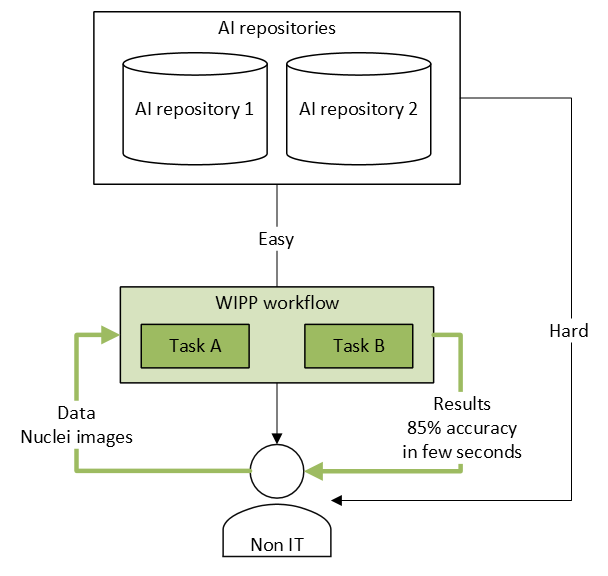
\includegraphics[width=0.8\linewidth]{png/introduction/layman.png}
\caption{Purpose of the work}
\end{figure}

Challenges are numerous: there is no
standard \Gls{API} to access public AI repositories; models are spread on
lot of different repositories and formats; re-train models from scratch take lot
of time and money; for non-technical researchers, it is not trivial to setup and
execute AI models; there is insufficient metadata about trained AI models in
public AI repositories to match them to applications and to run them; there
is no way of automatically assessing the accuracy of AI models.

Our motivations with this work is to accelerate application of AI models to
scientific problems and save hours of computation time by reusing pre-trained
models from diverse repositories.





\section{Methods}
\label{sec:methods}

\subsection{Related work}

There are already existing APIs or tools to download, inference and train AI
models:
\begin{itemize}
  \item Transformers (Hugging Face API) \cite{wolf-etal-2020-transformers}
  \item Cellpose API \cite{Stringer2020.02.02.931238}
  \item BioImage.IO Core (Python libraries)
  \item SAM2 repository \cite{ravi2024sam2}
\end{itemize}

The problem is there are no common APIs/CLIs/no standard.

For example with 'download API', there are 4 differents code for these 4 repositories:

\begin{listing}[H]
  \begin{minted}[frame=lines,framesep=2mm,baselinestretch=0.8,fontsize=\footnotesize,linenos]{python}
    # BioImage.IO
    model = load_description(args.model)

    # Hugging Face
    pipe = pipeline(task="mask-generation",
      model=args.model, points_per_batch=32,
      device=device)

    # SAM2
    mask_generator = SAM2AutomaticMaskGenerator
      .from_pretrained(args.model, device=device)
  \end{minted}

  \begin{minted}[frame=lines,framesep=2mm,baselinestretch=0.8,fontsize=\footnotesize,linenos]{bash}
    # Cellpose
    python -m cellpose --pretrained_model cyto3
  \end{minted}
\end{listing}

There is the same issue with 'inference API', 'train API', etc.

\subsection{Our approach}

We use existing APIs of AI repositories and use them in the context of WIPP. We
use AI model card to document AI model trained in WIPP.

Our contributions are:
\begin{itemize}
  \item Analyze API of AI repositories
  \item Implement them for containerized plugin that run in WIPP without learning the API
  \item Trained/Retrained AI model will comes with proper AI model card
\end{itemize}

\subsection{Web Image Processing Pipelines}

WIPP is a scientific workflow engine, illustrated as shown in figure 1.
The purpose of this tool is to make measurements based on terabyte-sized images.
It is an algorithmic plugin platform. Its goal is to lower the bar to execute
image analyses.

\begin{figure}[H]
  \centering
  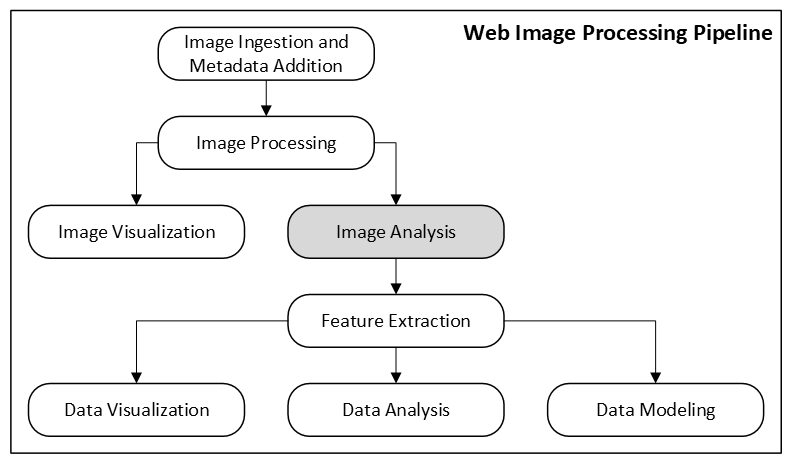
\includegraphics[width=1.0\linewidth]{png/1_wipp.png}
  \caption{\Gls{WIPP}}
  \label{fig:1wipp}
\end{figure}

WIPP worflows are sequence of plugins. WIPP plugins are piece of code (code put
in the form of a container) taking inputs and outputs and executing code.

Thanks to a plugin you can, for example, load an \Gls{AiModel} hosted in
\Gls{WIPP}, specify an
image collection and perform the \Gls{AiInference} of this \Gls{AiModel} on the
selected images.
The result will be a new collection of images modified by the \Gls{AiModel}, for
example
with a label after inference of a \Gls{ClassificationModel}.

\subsection{Access public \Gls{AiRepositories}}

There are many public AI models on lots of public AI repositories.

\begin{table}[H]
  \centering
  \caption{Number of models per repository}
  \begin{tabular}{lcc}
    \toprule
    AI repositories & IC models & S + MG models \\
    \midrule
    Hugging Face    & 15,593                      & 1,160 + 176 \\
    BioImage.IO     & 1                           & 4 + 32 \\
    Cellpose        & $\times$                    & 21 \\
    SAM2            & $\times$                    & 8 \\
    PyTorch Hub     & 20                          & 5 \\
    \bottomrule
  \end{tabular}
  \caption*{Image Classif. (IC), Segmentation (S), Mask Generation (MG)}
\end{table}

Our goal is to access external AI models in WIPP.


We have developed new inference plugins, see figure 2, to enable access to
\Gls{AiModel}s available on different public \Gls{AiRepositories} such as
Hugging Face, BioImage.IO, Cellpose, and more.

\begin{figure}[H]
  \centering
  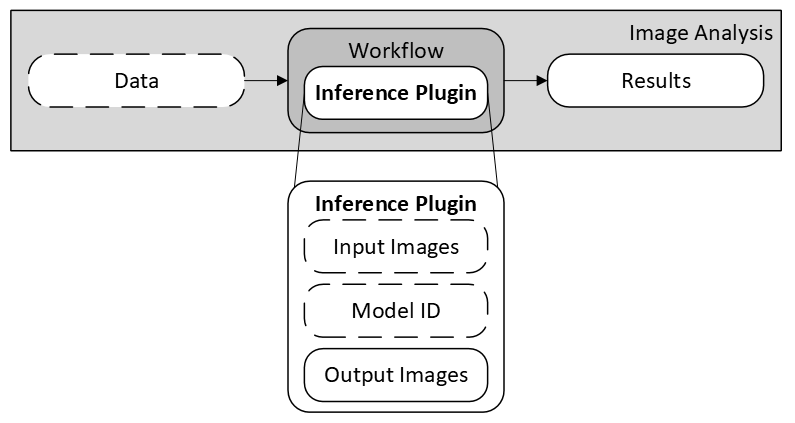
\includegraphics[width=1.0\linewidth]{png/2_inference_plugin.png}
  \caption{Inference Plugin}
  \label{fig:2inference}
\end{figure}

This was achieved by developing general-purpose code using the \Gls{API} of
the various platforms. This
enabled us to increase the number of \Gls{AiModel}s usable
in \Gls{WIPP} thanks to containerized software.

\subsection{Document \Gls{AiModel}s}

We have introduced \Gls{AiModelCard} entries that are necessary for matching tasks
with \Gls{AiModel}s. This information will also be needed as runtime parameters.
Figure 3, training an \Gls{AI} in \Gls{WIPP} automatically generates its documentation
(\Gls{AiModelCard}).

\begin{figure}[H]
  \centering
  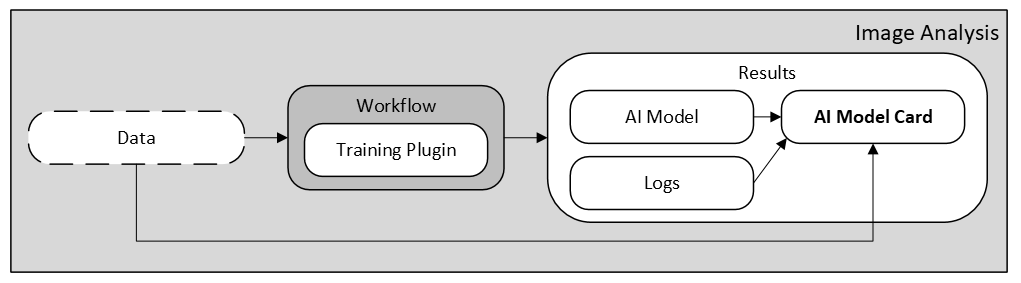
\includegraphics[width=1.0\linewidth]{png/3_ai_model_card.png}
  \caption{\Gls{AiModelCard}}
  \label{fig:3aimodelcard}
\end{figure}

This was achieved by developing code to retrieve information about the \Gls{AiModel}
throughout the pipeline: name, creation date, data used for training, number of
iterations, training time, and more.

\subsection{Compute accuracy}

Our goal is to mesure accuracy of external AI results and to select the most
accurate/fastest one.

We have developed a new plugin, see figure 4, to compute the \Gls{DiceIndex}.

The formula is:

\[ Dice = \frac{2*TP}{2*TP + FP + FN} \]

It is a statistic used to gauge the similarity of two samples, in
our case images.

\begin{figure}[H]
  \centering
  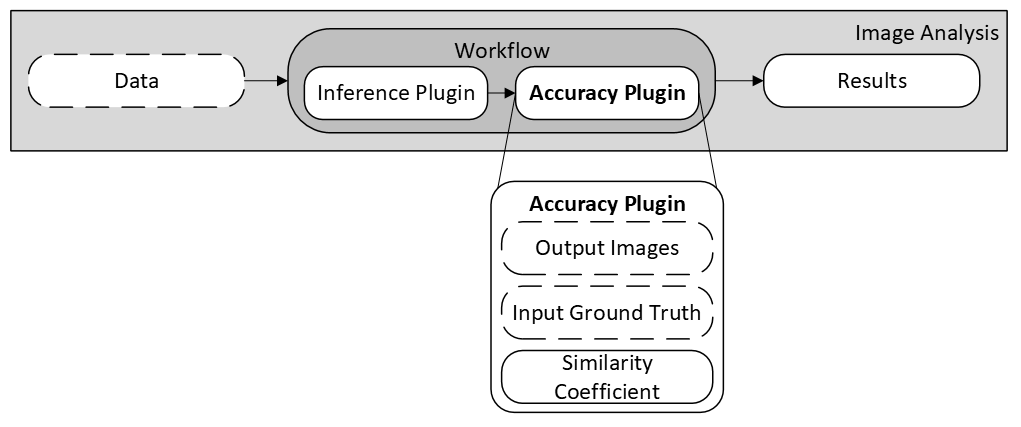
\includegraphics[width=1.0\linewidth]{png/4_accuracy.png}
  \caption{Accuracy Plugin}
  \label{fig:4accuracy}
\end{figure}

This was achieved by implementing the \Gls{DiceIndex}'s formula into a containerized
software (plugin). This makes it now possible to sequence model \Gls{AiInference} (a
model created within \Gls{WIPP} or a model from a repository) and evaluate the
accuracy of the result provided, by comparing it with
\Gls{GroundTruthData}.

\section{Results}
\label{sec:results}

\subsection{AI model cards}

The level of documentation varies greatly from model to model. We have set up an
automatic documentation system for models trained within \Gls{WIPP}.

\subsection{WIPP 2-steps workflow}

The WIPP 2-steps workflow is first, do the inference of the model and then
compute the accuracy.

\begin{figure}[H]
  \centering
  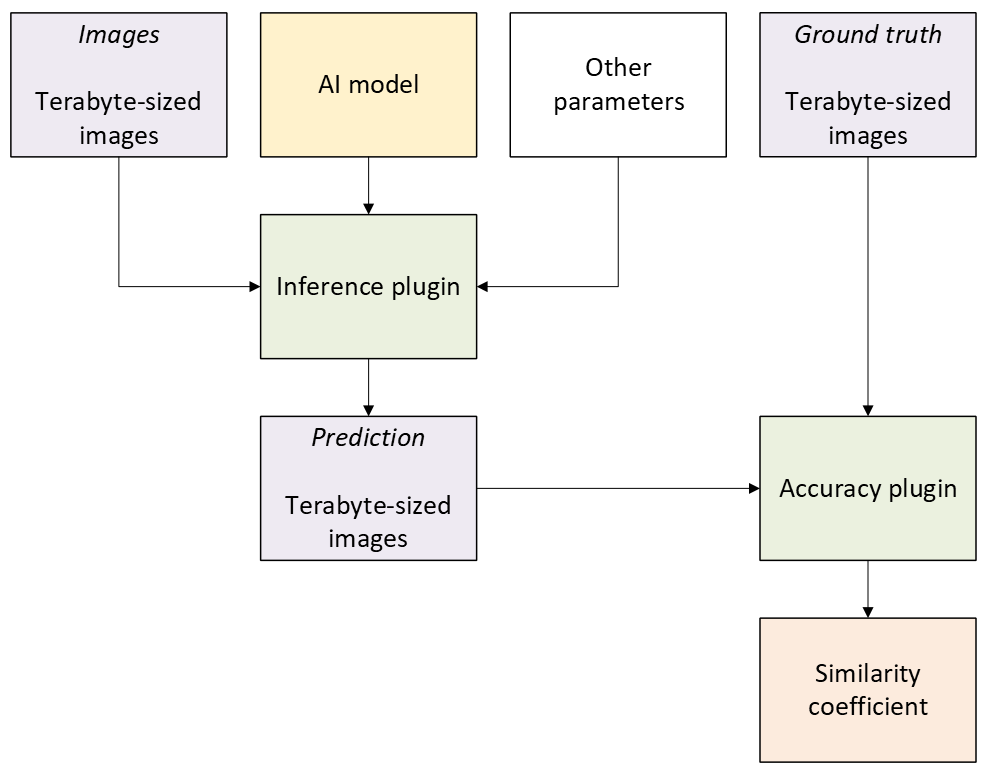
\includegraphics[width=1.0\linewidth]{png/results/workflow.png}
  \caption{WIPP 2-steps workflow}
  \label{fig:workflow}
\end{figure}

We compute everything in \Gls{WIPP}. The \Gls{WIPP} server specifications are:
\begin{itemize}
  \item CPU: AMD Ryzen 9 3950X 16-Core Processor with 2 threads
  \item GPU: NVIDIA GeForce RTX 3090
  \item 64G RAM
\end{itemize}

\subsection{Dataset 'cell boundary'}

We use the 'Retinal Pigment Epithelium' dataset. There are 1032 images of type
'cell microscopy' with size 256$\times$256.

\medskip

\begin{minipage}[h!]{0.20\textwidth}
  \centering
  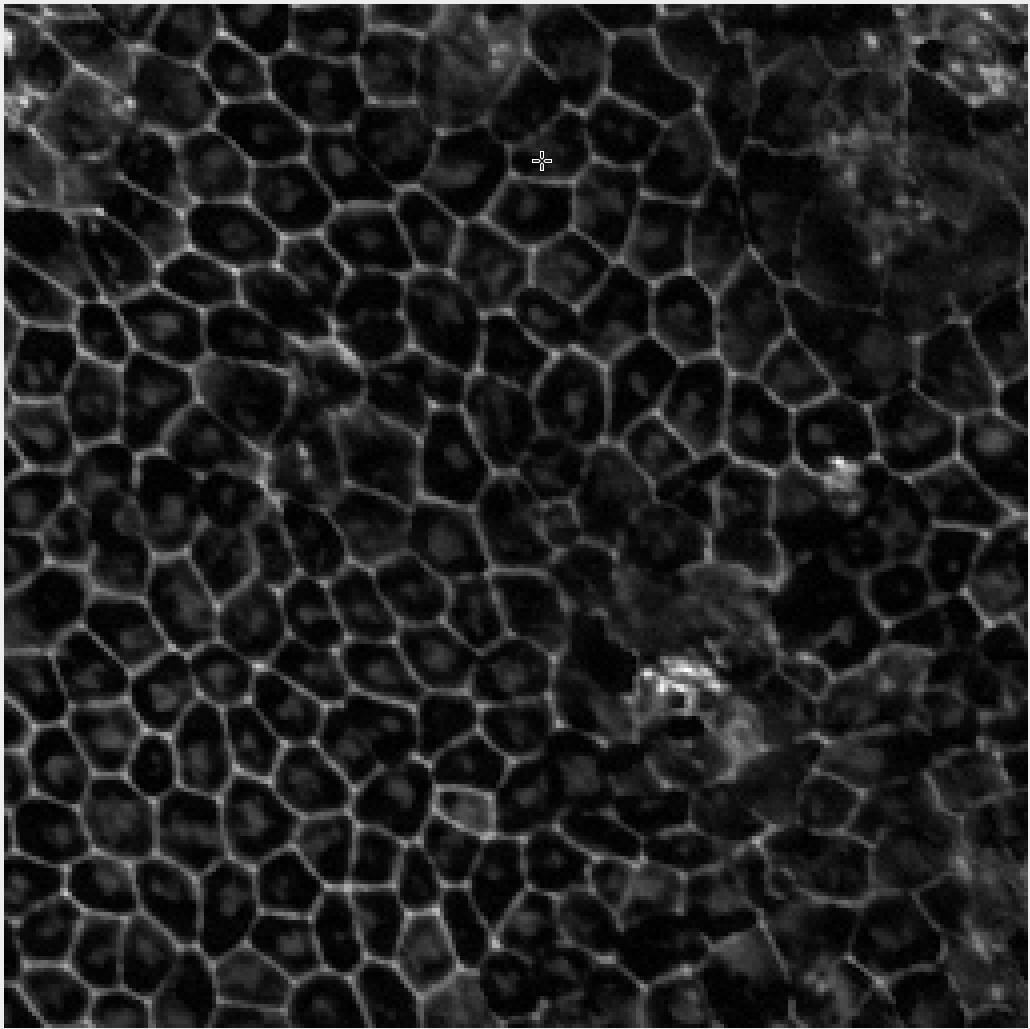
\includegraphics[scale=0.1]{./png/results/cell_image.png}
  \textbf{Image}
\end{minipage}\hfill
\begin{minipage}[h!]{0.20\textwidth}
  \centering
  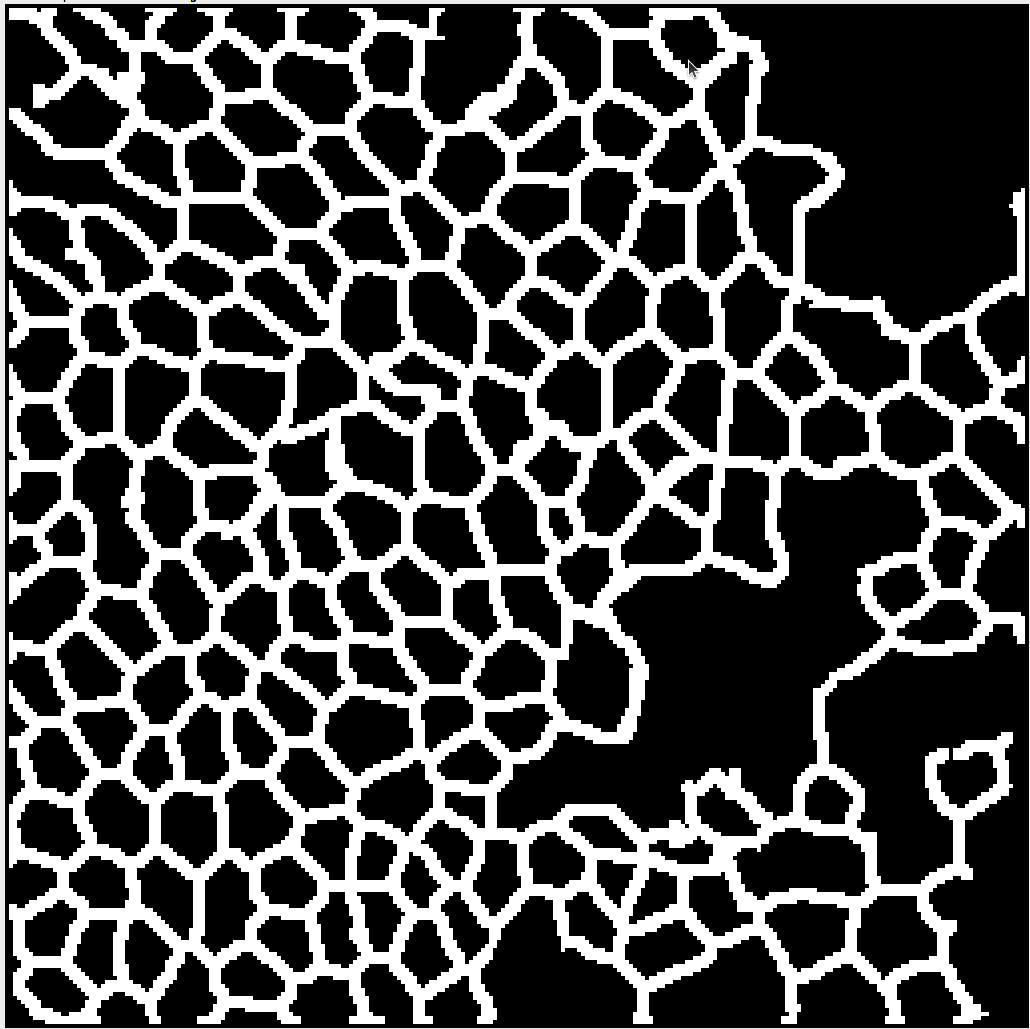
\includegraphics[scale=0.1]{./png/results/cell_mask.png}
  \textbf{Mask}
\end{minipage}

\medskip

Source: https://doi.org/doi:10.18434/T4/1503229

\subsection{Benchmark 'cell boundary'}

We inference different models to do the 'segments cell edges' task.

\begin{table}[H]
  \footnotesize
  \centering
  \caption{Accuracy after inference on data 'cell boundary'}
  \begin{tabular}{llcc}
    \toprule
    Repository    & Model                       & Accuracy             \\ [0.5ex]
    \midrule
    WIPP          & unet-cnn*                   & 95.11\% $\pm$ 0.78\% \\
    BioImage.IO   & 10.5281/zenodo.5869899      & 89.30\% $\pm$ 0.84\% \\
    Hugging Face  & facebook/sam-vit-huge       & 86.01\% $\pm$ 2.50\% \\
    SAM2          & facebook/sam2.1-hiera-large & 80.18\% $\pm$ 5.02\% \\
    Cellpose      & cyto3                       & 78.51\% $\pm$ 2.35\% \\
    \bottomrule
  \end{tabular}
  \caption*{*Trained then inferenced in WIPP}
\end{table}

\subsection{Dataset 'nuclei segmentation'}

We use the 'Kaggle 2018 Data Science Bowl' dataset. There are 497 images of type
'cell microscopy' with size 256$\times$256 and 696$\times$520.

\medskip

\begin{minipage}[h!]{0.20\textwidth}
  \centering
  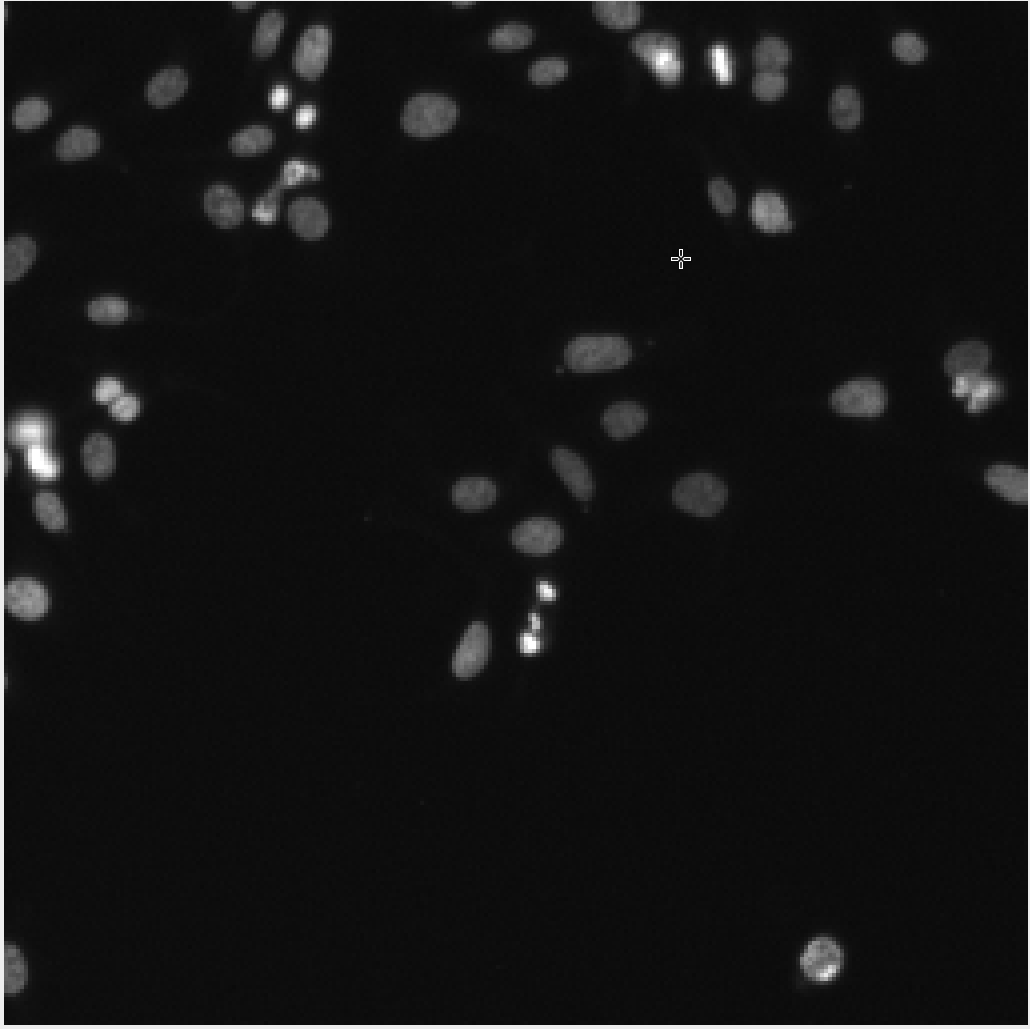
\includegraphics[scale=0.1]{./png/results/nuclei_image.png}
  \textbf{Image}
\end{minipage}\hfill
\begin{minipage}[h!]{0.20\textwidth}
  \centering
  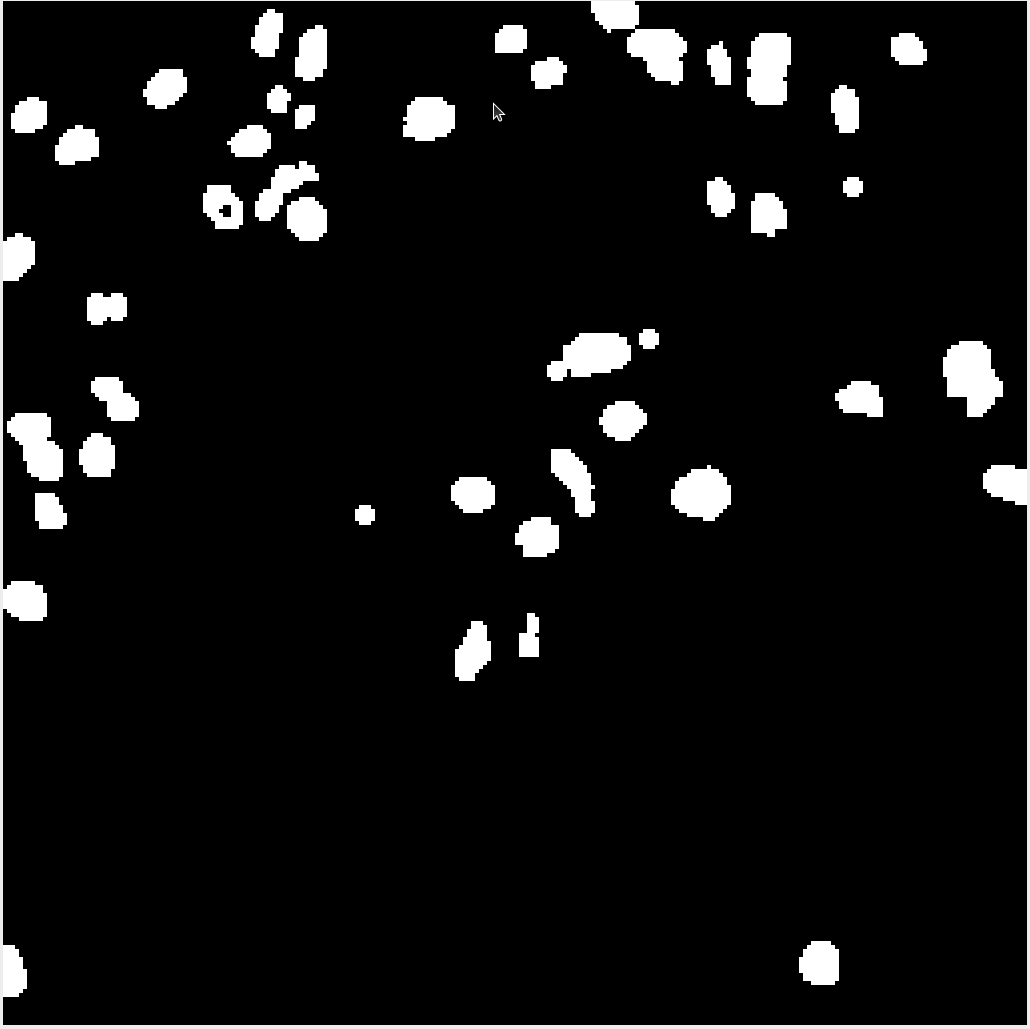
\includegraphics[scale=0.1]{./png/results/nuclei_mask.png}
  \textbf{Mask}
\end{minipage}

\medskip

Source: https://bbbc.broadinstitute.org/BBBC038/

\subsection{Benchmark 'nuclei segmentation'}

We inference different models to do the 'segments nuclei of cells' task.

\begin{table}[H]
  \footnotesize
  \centering
  \caption{Accuracy after inference on data 'nuclei segmentation'}
  \begin{tabular}{llcc}
    \toprule
    Repository    & Model                       & Accuracy               \\ [0.5ex]
    \midrule
    BioImage.IO  & 10.5281/zenodo.5764892        & 93.73\% $\pm$ 3.98\%  \\
    WIPP         & Stardist 2D paper DSB 2018*   & 90.67\% $\pm$ 4.42\%  \\
    Cellpose     & cyto3                         & 82.31\% $\pm$ 17.25\% \\
    Cellpose     & nuclei                        & 81.00\% $\pm$ 21.00\% \\
    SAM2         & facebook/sam2.1-hiera-small   & 48.18\% $\pm$ 32.41\% \\
    SAM2         & facebook/sam2.1-hiera-large   & 33.89\% $\pm$ 29.43\% \\
    BioImage.IO  & 10.5281/zenodo.5869899        & 29.47\% $\pm$ 8.32\%  \\
    Hugging Face & facebook/sam-vit-huge         & 21.63\% $\pm$ 15.37\% \\
    \bottomrule
  \end{tabular}
  \caption*{*Trained then inferenced in WIPP}
\end{table}

\subsection{Notes}

Even if the results may not be perfect, this method allows you to quickly try
out a new model at reduced cost. It is also easy to change dataset. We hope to
improve the speed of data analysis and enable better overall results.

\section{Discussion}
\label{sec:discussion}

\subsection{Public AI repositories}

There is no standard for the documentation and no standard for the usage.
It could be great to develop a standard
way to access AI models. This will allow to use more models from more different
repositories to give access to more people. For this paper we have tried to use
some repositories like below.

\begin{table}[H]
    \centering
    \caption{\label{tab:discussion}%
        Repositories not selected for this work
    }
    \begin{tabular}{lcccc}
      \toprule
      Repository & Mask Generation Model(s) \\
      \midrule
      PyTorch Hub & +50 \\
      Dinov2 & +10 \\
      Hailo.AI & 1 \\
      ModelZoo & 2 \\
      MicroSAM & +10 \\
      \bottomrule
    \end{tabular}
\end{table}

The lack of documentation, of APIs or of models available made it impossible to
use these repositories in WIPP. We hope to be able to integrate them into our
tool in the future.

\subsection{Documentation}

Documentation is also very important. Creating standard for AI model cards
could be great for the community.

In WIPP we have made decision by synthesizing the main AI model cards
already on the market:
\begin{itemize}
    \item Model Cards for Model Reporting, Google \cite{DBLP:journals/corr/abs-1810-03993}
    \item 
    \item 
    \item 
\end{itemize}



% \cite{MC_Paper}
% \cite{MC_HuggingFace}
% \cite{MC_BioImageIo}
% \cite{MC_Tensorflow}

\def\firstellip{(1.6, 0) ellipse [x radius=2.7cm, y radius=1.5cm, rotate=50]}
\def\secondellip{(0.3, 1cm) ellipse [x radius=2.7cm, y radius=1.5cm, rotate=50]}
\def\thirdellip{(-1.6, 0) ellipse [x radius=2.7cm, y radius=1.5cm, rotate=-50]}
\def\fourthellip{(-0.3, 1cm) ellipse [x radius=2.7cm, y radius=1.5cm, rotate=-50]}

\begin{figure}[H]
\centering
\begin{tikzpicture}

    \filldraw[fill=red,opacity=0.1] \firstellip;
    \filldraw[fill=blue,opacity=0.1] \secondellip;
    \filldraw[fill=green,opacity=0.1] \thirdellip;
    \filldraw[fill=yellow,opacity=0.1] \fourthellip;

    % TensorFlow (TF)
    \draw \firstellip node [label={[xshift=1.6cm, yshift=2.1cm] \tiny $TensorFlow$}] {};
    \draw node [label={[xshift=2.9cm, yshift=0.7cm] \tiny 26 fields}] {};

    % BioImage.IO (BI.IO)
    \draw \secondellip node [label={[xshift=1.5cm, yshift=2.1cm] \tiny $BioImage.IO$}] {};
    \draw node [label={[xshift=1.2cm, yshift=2.1cm] \tiny 53 fields}] {};

    % Hugging Face (HF)
    \draw \thirdellip node [label={[xshift=-1.6cm, yshift=2.1cm] \tiny $Hugging Face$}] {};
    \draw node [label={[xshift=-2.9cm, yshift=0.7cm] \tiny 43 fields}] {};

    % Google Paper (GP)
    \draw \fourthellip node [label={[xshift=-1.5cm, yshift=2.1cm] \tiny $Google Paper$}] {};
    \draw node [label={[xshift=-1.2cm, yshift=2.1cm] \tiny 30 fields}] {};

    % 
    \draw node [ label={ [xshift=-1.7cm,  yshift=1.2cm]   \tiny 16 fields} ] {};   % HF x GP
    \draw node [ label={ [xshift=1.7cm,   yshift=1.2cm]   \tiny 12 fields} ] {};   % BI.IO x TF
    \draw node [ label={ [xshift=0cm,     yshift=-1.9cm]  \tiny 15 fields} ] {};   % HF x TF
    \draw node [ label={ [xshift=-0.9cm,  yshift=0.2cm]   \small 10 fields} ] {};   % BI.IO x HF x GP
    \draw node [ label={ [xshift=0.9cm,   yshift=0.2cm]   \small 11 fields} ] {};   % BI.IO x TF x GP
    \draw node [ label={ [xshift=0cm,     yshift=-0.9cm]  \small  8 f.} ] {};   % HF x GP x BI.IO x TF

\end{tikzpicture}
\caption{Common field of different AI Model Cards} \label{fig:venn}
\end{figure}

This give us 8 fields that we want to keep to be as compatible as possible with
external tools. At the end we proposed an AI model card with 14 fields.

%\begin{itemize}
%    \item String: version
%    \item String: name
%    \item Date: date
%    \item String: framework
%    \item Map$\langle$String, String$\rangle$: trainingData
%    \item Map$\langle$String, String$\rangle$: trainingParameters
%    \item String: author
%    \item String: description
%    \item and more ...
%\end{itemize}

%For our needs, this works well, and
We manage to retrieve all this information automatically throughout the workflow.

%This proposal is not perfect and needs refinering.
The creation of a standard
would be a great opportunity for all the AI actors to think about what they
need.


%\begin{figure}[H]
%\centering
%\begin{tikzpicture}
%
%    \draw[draw=black] (-1.25,-1.25) rectangle ++(3.5, 3);
%    \filldraw[fill=red, opacity=0.1](0, 0) circle (1);
%    \filldraw[fill=blue, opacity=0.1](1, 0) circle (1);
%
%    \draw node [label={[xshift=0.5cm, yshift=-0.33cm] TP}] {};
%    \draw node [label={[xshift=0.5cm, yshift=1cm] TN}] {};
%    \draw node [label={[xshift=1.5cm, yshift=-0.33cm] FP}] {};
%    \draw node [label={[xshift=-0.5cm, yshift=-0.33cm] FN}] {};
%
%\end{tikzpicture}
%\caption{GT in red and PREDIC in blue} \label{fig:dice}
%\end{figure}





% DISCLAIMER: Certain commercial products or company names are identified here to describe our study adequately. Such identification is not intended to imply recommendation or endorsement by the National Institute of Standards and Technology, nor is it intended to imply that the products or names
% identified are necessarily the best available for the purpose.

{
    \small
    \bibliographystyle{ieeenat_fullname}
    \bibliography{main}
}
\printglossaries

% WARNING: do not forget to delete the supplementary pages from your submission
% \input{sec/X_suppl}

\end{document}
